%! TEX root = ../main.tex
\documentclass[main]{subfiles}

\begin{document}

\section{Reductions}
\label{sec:reduction}

Let $A$ be a discrete valuation ring with maximal ideal $\mathfrak{m}$ and fraction field $K$.
Assume that the residue field $k=A/\mathfrak{m}$ has $q=p^r$ elements with $p$ prime.
Let $S$ be an integral scheme with a morphism $S \to \Spec A$ that is projective and smooth of relative dimension $2$.
Then the projective surface $\overline{S}=S_{\overline{\mathbb{Q}}}$ and $\tilde{S}=S_{\overline{k}}$ are smooth over the algebraically closed field $\overline{\mathbb{Q}}$ and $\overline{k}$, respectively.
We will assume that $\overline{S}$ and $\tilde{S}$ are integrals, i.e., they are irreducible, nonsingular, projective surfaces.

For a prime number $l \neq p$, we denote by $H_{\text{\'et}}^{i}(\tilde{S}, \mathbb{Q}_l)$ the $l$-adic \'etale cohomology group of $X$ and by $H_{\text{\'et}}^{i}(\tilde{S}, \mathbb{Q}_l)(1)$ its Tate twist.

\begin{thm}{(\cite[Proposition 6.2.]{ref:vanluijk2007})}
    There are natural injective homomorphisms
    \begin{equation*}
        \NS (\overline{S}) \otimes_{\mathbb{Z}} \mathbb{Q}_{l} \hookrightarrow \NS (\tilde{S}) \otimes_{\mathbb{Z}} \mathbb{Q}_{l} \hookrightarrow H_{\text{\'et}}^{2}(\tilde{S}, \mathbb{Q}_{l}(1)) = H_{\text{\'et}}^{2}(\tilde{S}, \mathbb{Q}_{l})(1)
    \end{equation*}
    of finite-dimensional vector spaces over $\mathbb{Q}_l$.
\end{thm}

Let $F: S_k \to S_k$ denote the absolute Frobenius, which acts as the identity on points and by $f \mapsto f^p$ on the structure sheaf.
Set $\varphi:=F^{r}$ where $r$ is the integer such that $q=p^r$, and let $\varphi^{(i)}$ denote the automorphism on $H_{\text{\'et}}^{i}(\tilde{S}, \mathbb{Q}_l)$ induced by $\varphi \times 1$ acting on $S_k \times_{\Spec k} \Spec \overline{k} \cong \tilde{S}$.

\begin{cor}{(\cite[Corollary 6.4.]{ref:vanluijk2007})}
    \label{cor:ns_upper_bound}
    The ranks of $\NS (\overline{S})$ and $\NS (\tilde{S})$ are bounded from above by the number of eigenvalues $\lambda$ of $\varphi^{(2)}$ for which $\lambda/q$ is a root of unity, counted with multiplicity.
\end{cor}

\begin{rem}{(\cite[Remark 6.5.]{ref:vanluijk2007})}
    Tate's conjecture states that the upper bound mentioned in Corollary~\ref{cor:ns_upper_bound} is actually equal to the rank of $\NS (\tilde{S})$.
    Tate's conjecture was proven for elliptic K3 surfaces by Artin and Swinnerton-Dyer \cite{ref:Artin1973}.
\end{rem}

Now we want to calculate the characteristic polynomial $\chara (\varphi^{(2)})$.
Beforehand, we recall the Lefschetz fixed point theorem.

\begin{thm}
    \label{thm:lefschetz}
    \begin{equation*}
        \# \tilde{S}(\mathbb{F}_{q^{m}}) = \sum_{i = 0}^{n} ( - 1)^{i} \Tr((\varphi^{(i)})^{m})
    \end{equation*}
\end{thm}

\begin{cor}
    \label{cor:lefschetz}
    \begin{equation*}
        \Tr ((\varphi^{(2)})^{m}) = \# \tilde{S}(\mathbb{F}_{q^{m}}) - 1 - q^{2m}
    \end{equation*}
\end{cor}
\begin{proof}
    Since
    \begin{equation*}
        \dim H_{\text{\'et}}^{1}(\tilde{S}, \mathbb{Q}_{l}) = \dim H_{\text{\'et}}^{3}(\tilde{S}, \mathbb{Q}_{l}) = 0
    \end{equation*}
    and $\varphi^{(4)}$ acts on $H_{\text{\'et}}^{4}(\tilde{S}, \mathbb{Q}_l) \cong \mathbb{Q}_l$ by multiplication by $q^{2}$,
    we get the conclusion from Theorem~\ref{thm:lefschetz}.
\end{proof}

Let $V$ be the linear subspace of $H_{\text{\'et}}^{2}(\tilde{S}, \mathbb{Q}_{l})$ generated by the components of the singular fibers and by the zero section and $W = H_{\text{\'et}}^{2}(\tilde{S}, \mathbb{Q}_l) / V$, then
\begin{equation}
    \label{eq:dimV}
    \dim V = \sum_{v \in R} (m_{v} - 1) + 2.
\end{equation}
By the multiplicativity of the characteristic polynomial, we have
\begin{equation*}
    \chara (\varphi^{(2)}) = \chara (\varphi^{(2)} | V) \cdot \chara (\varphi^{(2)}_{W})
\end{equation*}
and
\begin{equation}
    \Tr ((\varphi^{(2)})^{m}) = \Tr ((\varphi^{(2)} | V)^{m}) + \Tr ((\varphi^{(2)}_{W})^{m}) \label{eq:trcomposition}
\end{equation}
for any $m \in \mathbb{Z}$, where $\varphi^{(2)}_W: W \to W$ is induced by $\varphi^{(2)}$.
Since $\varphi^{(2)}$ acts on $V$ by multiplication by $q$, we have
\begin{equation*}
    \chara (\varphi^{(2)} | V) = (x - q)^{\dim V}.
\end{equation*}

As for the characteristic polynomial of $\varphi^{(2)}_{W}$, let $t_{m} := \Tr((\varphi^{(2)}_{W})^{m})$, then $\chara (\varphi^{(2)}_{W})$ is the polynomial part of
\begin{equation*}
    \frac{x^{\dim W}}{\exp \left( \sum_{m = 1}^{\infty} \frac{t_{m}}{m} x^{-m} \right)} = x^{\dim W} \left( 1 + t_{1} x^{-1} + \frac{t_{1}^{2} - t^{2}}{2} x^{-2} + \frac{-t_{1}^{3} + 3 t_{1} t_{2} - 2 t_{3}}{6} x^{-3} + \cdots \right).
\end{equation*}
Here, by \eqref{eq:trcomposition} and Corollary~\ref{cor:lefschetz}, we have
\begin{equation*}
    t_{m} = \# \tilde{S}(\mathbb{F}_{q^{m}}) - 1 - q^{2m} - \dim V \cdot q^{m}.
\end{equation*}

\begin{lem}{(\cite[Theorem 4, Part III]{ref:mumford2004})}
    \label{lem:k3-betti}
    If $\tilde{S}$ is a elliptic K3 surface, then the second Betti number of $\tilde{S}$ is $22$.
\end{lem}

\begin{thm}
    \begin{equation*}
        \rank E_{0,u}^{(1 + 3u)}(\overline{\mathbb{Q}}(u)) = 0
    \end{equation*}
\end{thm}
\begin{proof}
    We denote by $S=\mathcal{E}_{0,u}^{(1 + 3u)} \to \mathbb{P}^1$ the elliptic surface with the generic fiber $E_{0,u}^{(1 + 3u)}$.
    The discriminant of $E_{0,u}^{(1 + 3u)}$ is
    \begin{equation*}
        \Delta_{E_{0,u}^{(1 + 3u)}} = 256 u^2 (u - 1)^4 (u + 1)^4 (3u + 1)^6
    \end{equation*}
    and the types of the singular fibers of $E_{0,u}^{(1 + 3u)}$ are calculated as in Table~\ref{tab:E_{0,u}^{(1 + 3u)}} by Tate's algorithm.
    Put $\mathfrak{p}=(5) \in \Spec \mathbb{Z}$ and $A = \mathbb{Z}_{\mathfrak{p}}$.
    The residue field $k=A/\mathfrak{p} \cong \mathbb{F}_{5}$.
    $S$ defines an elliptic surface $\tilde{S} = S_{\overline{\mathbb{F}_{5}}} \to \mathbb{P}^1$.
    We can check that $\tilde{S}$ has exactly the same types of singular fibers as $S$.

    \begin{table}[H]
        \centering
        \caption{Singular fibers of $E_{0,u}^{(1 + 3u)}$}
        \begin{tabular}{|c|c|c|c|}
            \hline
            Place            & Type    & $m_v$ & $e$ \\
            \hline
            $u=0$            & $I_2$   & 2     & 2   \\
            $u=\pm 1$        & $I_4$   & 4     & 4   \\
            $u=-\frac{1}{3}$ & $I_0^*$ & 5     & 6   \\
            $u=\infty$       & $I_2^*$ & 7     & 8   \\
            \hline
        \end{tabular}
        \label{tab:E_{0,u}^{(1 + 3u)}}
    \end{table}
    Then since $e(\tilde{S})=2+4 \times2+6+8=24$, $\tilde{S}$ is a elliptic K3 surface and by Lemma~\ref{lem:k3-betti}, we have
    \begin{equation*}
        \dim_{\mathbb{Q}_{l}} H_{\text{\'et}}^{2}(\tilde{S}, \mathbb{Q}_{l}) = 22.
    \end{equation*}
    The subspace $V$ is of rank 19 by \eqref{eq:dimV}, on which the Frobenius automorphism acts by multiplication by $5$.
    Thus
    \begin{equation*}
        \chara (\varphi^{(2)} | V) = (x - 5)^{19}
    \end{equation*}

    In order to calculate the characteristic polynomial of $\varphi^{(2)}_{W}$, we need to compute the number of points on $\tilde{S}$ over finite fields $\mathbb{F}_{5^{m}}$.
    Note that all the multiplicative fibers are split in $\mathbb{F}_{5^{m}}$ for $m=1,2,3$.
    We count the number of points on each special fibers.
    For non-singular fibers, the Schoof-Elkies-Atkin (SEA) algorithm, which calculates the number of points on an elliptic curve over a finite field, is known and can be used.
    For each singular fiber, the number of points is determined by the type of the fiber.
    Singular fibers' configurations are as shown in Table~\ref{tab:reductionpoints} where each component is $\mathbb{P}^{1}$.
    We get the number of points by subtracting from $m_v \times \#\mathbb{P}^1(\mathbb{F}_{q^m}) = m_v(q^m + 1)$ the number of points that are counted twice or more.
    \begin{table}[H]
        \centering
        \caption{Number of points on each singular fiber over a finite field}
        \begin{tabular}{|c|c|c|c|}
            \hline
            Type             & Configuration                                                                      & $m_v$ & $\mathcal{E}_v(\mathbb{F}_{q^{m}})$ \\
            \hline
            $\mathrm{I}_n$   & \raisebox{-0.5 \height}{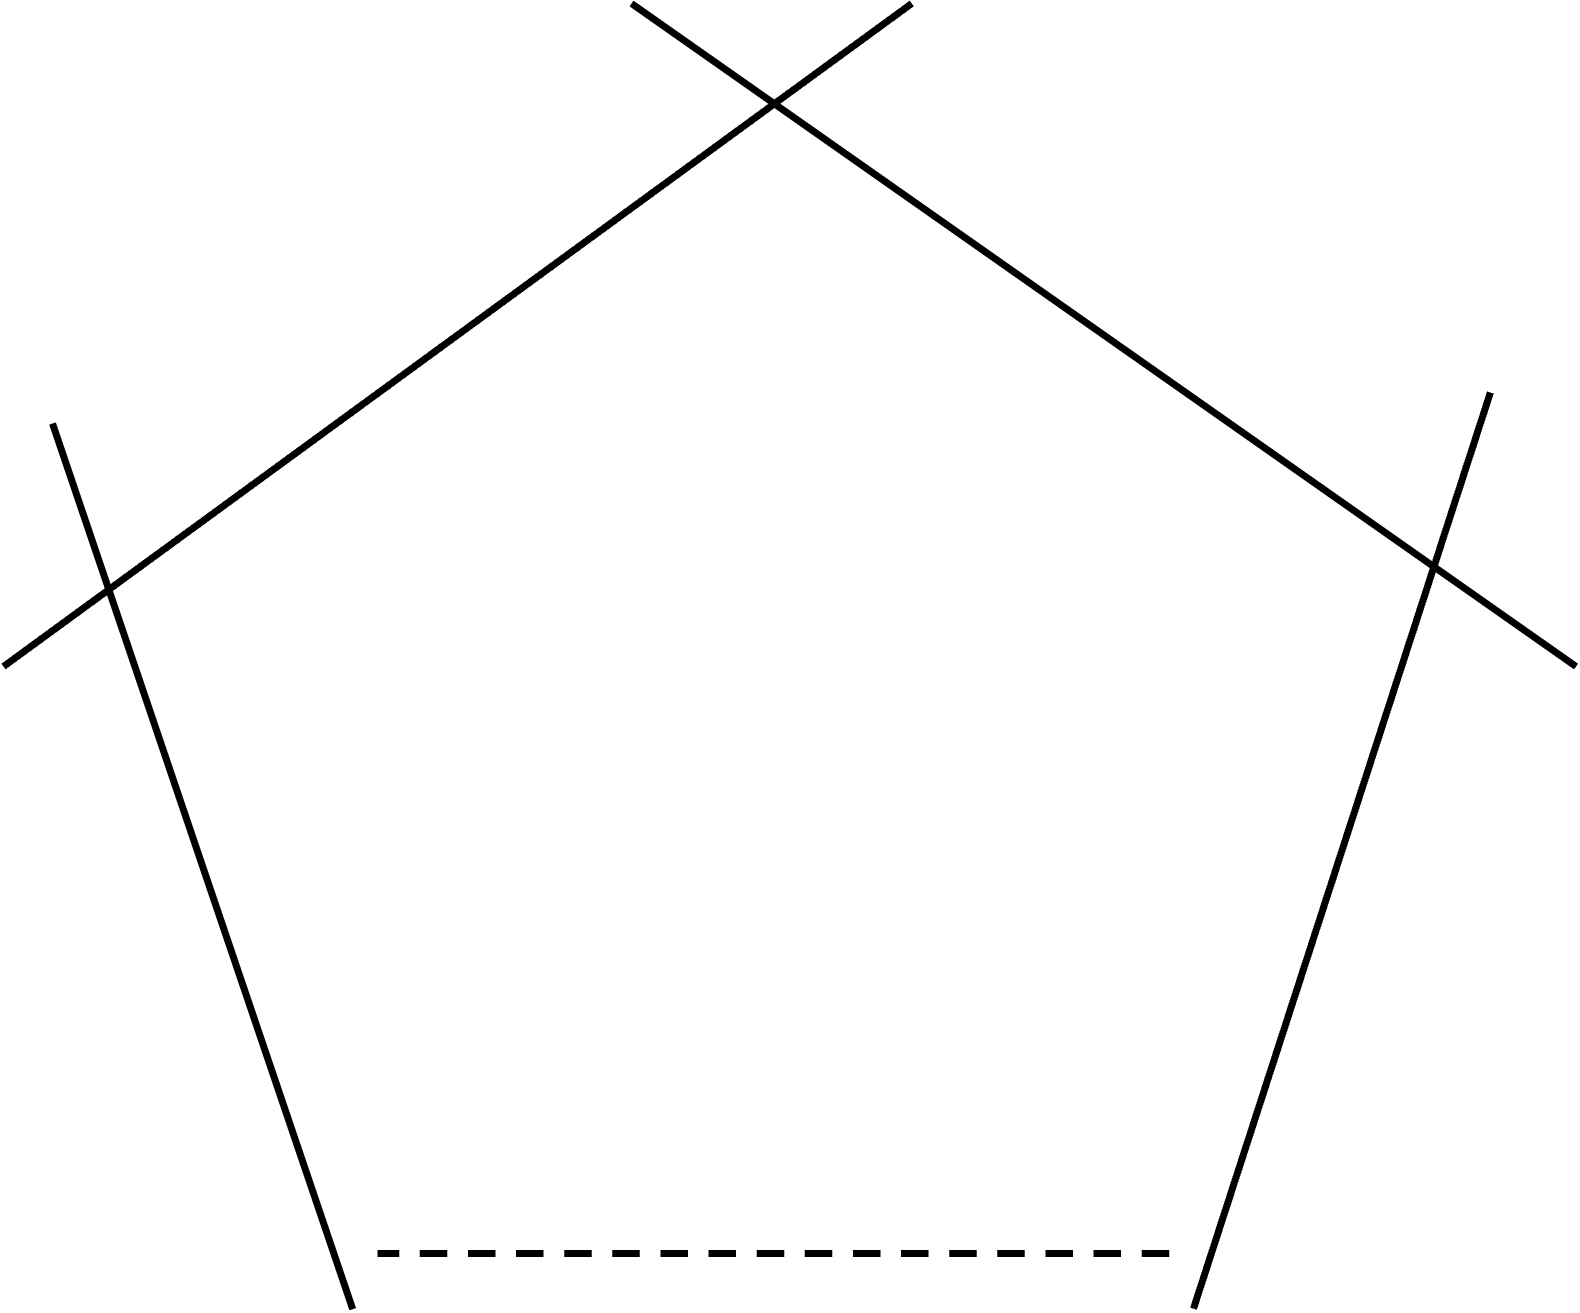
\includegraphics[width=4cm, height=3cm]{figures/I_n.png}}  & $n$   & $nq^m$                              \\
            $\mathrm{I}_n^*$ & \raisebox{-0.5 \height}{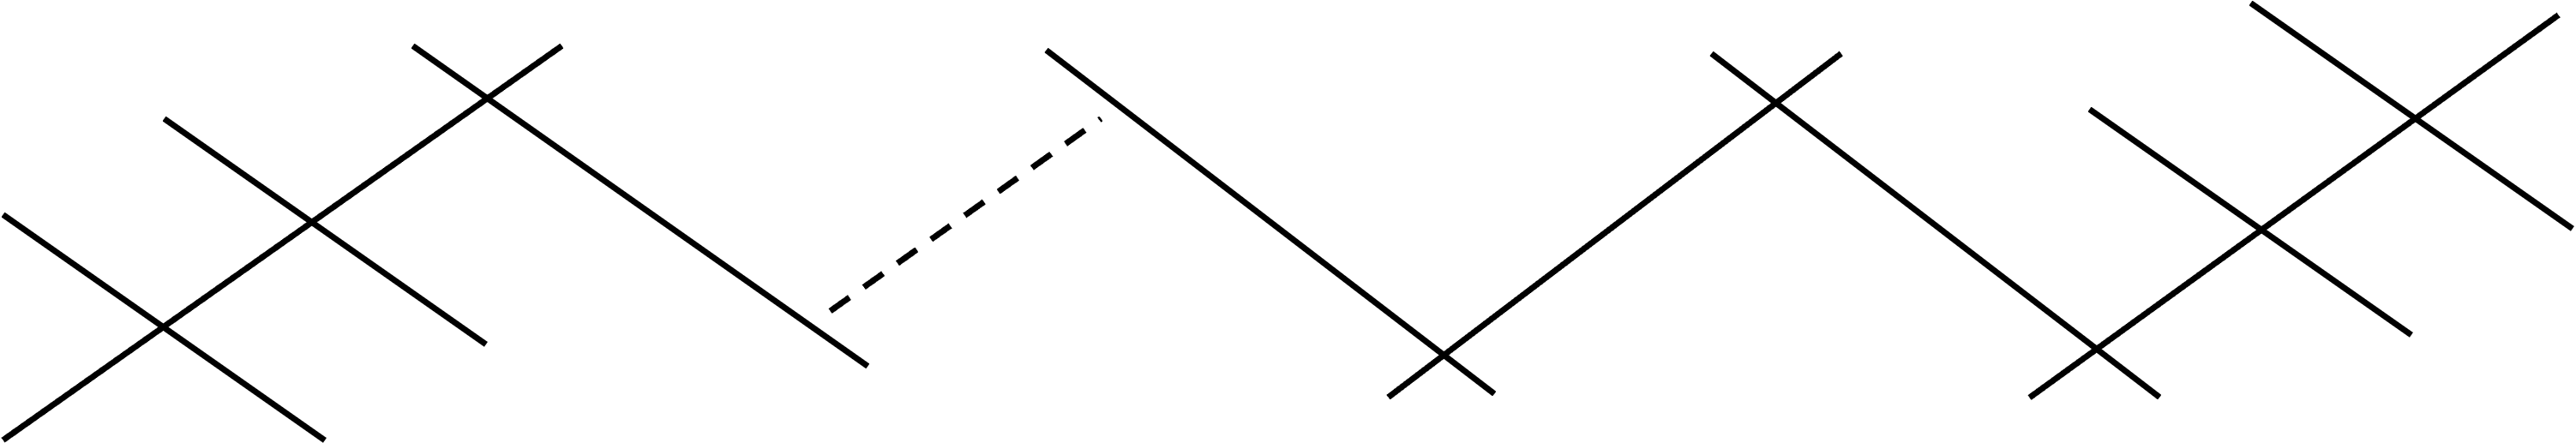
\includegraphics[width=4cm, height=2cm]{figures/I_nx.png}} & $n+5$ & $(n+5) q^m+1$                       \\
            \hline
        \end{tabular}
        \label{tab:reductionpoints}
    \end{table}
    
    \begin{equation*}
        t_{m} = \# \tilde{S}(\mathbb{F}_{5^{m}}) - 1 - 5^{2m} - 19 \cdot 5^{m}.
    \end{equation*}

    These calculations result in Table~\ref{tab:tm}.
    \begin{table}[H]
        \centering
        \caption{$\# \tilde{S}(\mathbb{F}_{5^{m}})$ and $t_{m}$}
        \begin{tabular}{|c|c|c|c|}
            \hline
            $m$                              & 1   & 2    & 3     \\
            \hline
            $\# \tilde{S}(\mathbb{F}_{5^m})$ & 120 & 1080 & 18264 \\
            \hline
            $t_m$                            & -1  & -21  & 263   \\
            \hline
        \end{tabular}
        \label{tab:tm}
    \end{table}

    Therefore, we have
    \begin{equation*}
        \chara(\varphi_{W}^{(2)}) = x^{3} + x^{2} + 11 x - 77.
    \end{equation*}

    If $\chara (\varphi_{W}^{(2)})$ has a root of the form $x=5 \zeta$ for some root of unity $\zeta$, then $\zeta$ is a root of the polynomial
    \begin{equation*}
        125x^{3} + 25x^{2} + 55 x - 77,
    \end{equation*}
    which is irreducible over $\mathbb{Q}$.
    It contradicts the fact that $\zeta$ is an algebraic integer.
    By Corollary~\ref{cor:ns_upper_bound}, $\rho(\mathcal{E}_{0,u}^{(1 + 3u)}) \leq 19$.
    Then by Theorem~\ref{thm:shioda}, we have
    \begin{equation*}
        \rank E_{0,u}^{(1 + 3u)}(\overline{\mathbb{Q}}(u)) \leq 19 - (2 + (2 - 1) + (4 - 1) \times 2 + (5 - 1) + (7 - 1)) = 0.
    \end{equation*}
\end{proof}

This concludes the proof of the main theorem.

\end{document}
